% Options for packages loaded elsewhere
\PassOptionsToPackage{unicode}{hyperref}
\PassOptionsToPackage{hyphens}{url}
%
\documentclass[
]{book}
\usepackage{amsmath,amssymb}
\usepackage{iftex}
\ifPDFTeX
  \usepackage[T1]{fontenc}
  \usepackage[utf8]{inputenc}
  \usepackage{textcomp} % provide euro and other symbols
\else % if luatex or xetex
  \usepackage{unicode-math} % this also loads fontspec
  \defaultfontfeatures{Scale=MatchLowercase}
  \defaultfontfeatures[\rmfamily]{Ligatures=TeX,Scale=1}
\fi
\usepackage{lmodern}
\ifPDFTeX\else
  % xetex/luatex font selection
\fi
% Use upquote if available, for straight quotes in verbatim environments
\IfFileExists{upquote.sty}{\usepackage{upquote}}{}
\IfFileExists{microtype.sty}{% use microtype if available
  \usepackage[]{microtype}
  \UseMicrotypeSet[protrusion]{basicmath} % disable protrusion for tt fonts
}{}
\makeatletter
\@ifundefined{KOMAClassName}{% if non-KOMA class
  \IfFileExists{parskip.sty}{%
    \usepackage{parskip}
  }{% else
    \setlength{\parindent}{0pt}
    \setlength{\parskip}{6pt plus 2pt minus 1pt}}
}{% if KOMA class
  \KOMAoptions{parskip=half}}
\makeatother
\usepackage{xcolor}
\usepackage{color}
\usepackage{fancyvrb}
\newcommand{\VerbBar}{|}
\newcommand{\VERB}{\Verb[commandchars=\\\{\}]}
\DefineVerbatimEnvironment{Highlighting}{Verbatim}{commandchars=\\\{\}}
% Add ',fontsize=\small' for more characters per line
\usepackage{framed}
\definecolor{shadecolor}{RGB}{248,248,248}
\newenvironment{Shaded}{\begin{snugshade}}{\end{snugshade}}
\newcommand{\AlertTok}[1]{\textcolor[rgb]{0.94,0.16,0.16}{#1}}
\newcommand{\AnnotationTok}[1]{\textcolor[rgb]{0.56,0.35,0.01}{\textbf{\textit{#1}}}}
\newcommand{\AttributeTok}[1]{\textcolor[rgb]{0.13,0.29,0.53}{#1}}
\newcommand{\BaseNTok}[1]{\textcolor[rgb]{0.00,0.00,0.81}{#1}}
\newcommand{\BuiltInTok}[1]{#1}
\newcommand{\CharTok}[1]{\textcolor[rgb]{0.31,0.60,0.02}{#1}}
\newcommand{\CommentTok}[1]{\textcolor[rgb]{0.56,0.35,0.01}{\textit{#1}}}
\newcommand{\CommentVarTok}[1]{\textcolor[rgb]{0.56,0.35,0.01}{\textbf{\textit{#1}}}}
\newcommand{\ConstantTok}[1]{\textcolor[rgb]{0.56,0.35,0.01}{#1}}
\newcommand{\ControlFlowTok}[1]{\textcolor[rgb]{0.13,0.29,0.53}{\textbf{#1}}}
\newcommand{\DataTypeTok}[1]{\textcolor[rgb]{0.13,0.29,0.53}{#1}}
\newcommand{\DecValTok}[1]{\textcolor[rgb]{0.00,0.00,0.81}{#1}}
\newcommand{\DocumentationTok}[1]{\textcolor[rgb]{0.56,0.35,0.01}{\textbf{\textit{#1}}}}
\newcommand{\ErrorTok}[1]{\textcolor[rgb]{0.64,0.00,0.00}{\textbf{#1}}}
\newcommand{\ExtensionTok}[1]{#1}
\newcommand{\FloatTok}[1]{\textcolor[rgb]{0.00,0.00,0.81}{#1}}
\newcommand{\FunctionTok}[1]{\textcolor[rgb]{0.13,0.29,0.53}{\textbf{#1}}}
\newcommand{\ImportTok}[1]{#1}
\newcommand{\InformationTok}[1]{\textcolor[rgb]{0.56,0.35,0.01}{\textbf{\textit{#1}}}}
\newcommand{\KeywordTok}[1]{\textcolor[rgb]{0.13,0.29,0.53}{\textbf{#1}}}
\newcommand{\NormalTok}[1]{#1}
\newcommand{\OperatorTok}[1]{\textcolor[rgb]{0.81,0.36,0.00}{\textbf{#1}}}
\newcommand{\OtherTok}[1]{\textcolor[rgb]{0.56,0.35,0.01}{#1}}
\newcommand{\PreprocessorTok}[1]{\textcolor[rgb]{0.56,0.35,0.01}{\textit{#1}}}
\newcommand{\RegionMarkerTok}[1]{#1}
\newcommand{\SpecialCharTok}[1]{\textcolor[rgb]{0.81,0.36,0.00}{\textbf{#1}}}
\newcommand{\SpecialStringTok}[1]{\textcolor[rgb]{0.31,0.60,0.02}{#1}}
\newcommand{\StringTok}[1]{\textcolor[rgb]{0.31,0.60,0.02}{#1}}
\newcommand{\VariableTok}[1]{\textcolor[rgb]{0.00,0.00,0.00}{#1}}
\newcommand{\VerbatimStringTok}[1]{\textcolor[rgb]{0.31,0.60,0.02}{#1}}
\newcommand{\WarningTok}[1]{\textcolor[rgb]{0.56,0.35,0.01}{\textbf{\textit{#1}}}}
\usepackage{longtable,booktabs,array}
\usepackage{calc} % for calculating minipage widths
% Correct order of tables after \paragraph or \subparagraph
\usepackage{etoolbox}
\makeatletter
\patchcmd\longtable{\par}{\if@noskipsec\mbox{}\fi\par}{}{}
\makeatother
% Allow footnotes in longtable head/foot
\IfFileExists{footnotehyper.sty}{\usepackage{footnotehyper}}{\usepackage{footnote}}
\makesavenoteenv{longtable}
\usepackage{graphicx}
\makeatletter
\def\maxwidth{\ifdim\Gin@nat@width>\linewidth\linewidth\else\Gin@nat@width\fi}
\def\maxheight{\ifdim\Gin@nat@height>\textheight\textheight\else\Gin@nat@height\fi}
\makeatother
% Scale images if necessary, so that they will not overflow the page
% margins by default, and it is still possible to overwrite the defaults
% using explicit options in \includegraphics[width, height, ...]{}
\setkeys{Gin}{width=\maxwidth,height=\maxheight,keepaspectratio}
% Set default figure placement to htbp
\makeatletter
\def\fps@figure{htbp}
\makeatother
\setlength{\emergencystretch}{3em} % prevent overfull lines
\providecommand{\tightlist}{%
  \setlength{\itemsep}{0pt}\setlength{\parskip}{0pt}}
\setcounter{secnumdepth}{5}
\usepackage{booktabs}
\ifLuaTeX
  \usepackage{selnolig}  % disable illegal ligatures
\fi
\usepackage[]{natbib}
\bibliographystyle{plainnat}
\IfFileExists{bookmark.sty}{\usepackage{bookmark}}{\usepackage{hyperref}}
\IfFileExists{xurl.sty}{\usepackage{xurl}}{} % add URL line breaks if available
\urlstyle{same}
\hypersetup{
  pdftitle={Laboratorio di agronomia di precisione},
  pdfauthor={Michele Croci},
  hidelinks,
  pdfcreator={LaTeX via pandoc}}

\title{Laboratorio di agronomia di precisione}
\author{Michele Croci}
\date{2024-06-13}

\usepackage{amsthm}
\newtheorem{theorem}{Theorem}[chapter]
\newtheorem{lemma}{Lemma}[chapter]
\newtheorem{corollary}{Corollary}[chapter]
\newtheorem{proposition}{Proposition}[chapter]
\newtheorem{conjecture}{Conjecture}[chapter]
\theoremstyle{definition}
\newtheorem{definition}{Definition}[chapter]
\theoremstyle{definition}
\newtheorem{example}{Example}[chapter]
\theoremstyle{definition}
\newtheorem{exercise}{Exercise}[chapter]
\theoremstyle{definition}
\newtheorem{hypothesis}{Hypothesis}[chapter]
\theoremstyle{remark}
\newtheorem*{remark}{Remark}
\newtheorem*{solution}{Solution}
\begin{document}
\maketitle

{
\setcounter{tocdepth}{1}
\tableofcontents
}
\hypertarget{prefazione}{%
\chapter{Prefazione}\label{prefazione}}

Benvenuti in un viaggio entusiasmante, dove scienza dei dati, statistica e agronomia si incontrano per andare verso il futuro dell'agricoltura. Questo corso introduttivo, progettato per studenti delle scienze agrarie, vi guiderà attraverso esercitazioni pratiche di analisi dati per affrontare le sfide quotidiane nel campo della ricerca e della produzione agricola.

L'\textbf{analisi dei dati} è diventata un pilastro fondamentale nella scienza moderna, aprendo nuove strade per soluzioni innovative, analisi approfondite e la garanzia di risultati riproducibili. Questo materiale, appositamente creato per studenti con poca o nessuna esperienza di analisi dati, vi accompagnerà passo dopo passo in questa avventura, partendo dai concetti base fino a raggiungere un livello di competenza che vi permetterà di esplorare, visualizzare, modellare e interpretare dati complessi.

R, il linguaggio scelto per questo percorso, è rinomato per la sua potenza nel campo della statistica e dell'analisi dati, nonché per la sua vasta adozione nella comunità scientifica. Grazie ad un ricco ecosistema di pacchetti e strumenti dedicati, R rende l'analisi dei dati accessibile e potente. Il codice presentato, affiancato da lezioni pratiche, vi familiarizzerà gradualmente con la sintassi di R, le sue funzioni principali e l'arte di trasformare dati grezzi in informazioni significative.

Il nostro obiettivo è quello di fornire un approccio equilibrato, combinando la complessità delle analisi con un uso oculato dei pacchetti. Sebbene i pacchetti offrano indubbi vantaggi in termini di efficienza e funzionalità, un eccessivo affidamento ad essi può ostacolare la comprensione dei concetti fondamentali dell'analisi dati. Attraverso l'utilizzo di dati reali provenienti da studi e progetti di ricerca, questo corso colma il divario tra teoria e pratica, offrendo esempi concreti e applicabili per consolidare le vostre competenze.

Nel corso della mia carriera, ho sperimentato in prima persona come l'analisi dei dati possa rivelare pattern nascosti, guidare decisioni informate e fornire una comprensione più profonda dei fenomeni agronomici. Spero sinceramente che possiate trovare in queste pagine non solo un percorso di apprendimento, ma anche un'autentica passione per l'analisi dei dati.

Benvenuti nel mondo dell'analisi dati applicata all'agronomia. Buon divertimento!

\textbf{Michele Croci}\\
Assistant Professor in Agronomy \& Field Crops\\
Department of Sustainable Crop Production\\
Università Cattolica del Sacro Cuore

\hypertarget{coltivazioni-erbacee}{%
\chapter{Coltivazioni erbacee}\label{coltivazioni-erbacee}}

\hypertarget{introduzione}{%
\section{Introduzione}\label{introduzione}}

Il corso di coltivazioni erbacee mira a fornire una conoscenza approfondita delle tecniche colturali relative alle specie erbacee di pieno campo, evidenziandone l'importanza nel contesto agricolo italiano ed europeo. L'obiettivo principale è acquisire competenze nella gestione delle principali coltivazioni, tenendo conto non solo degli aspetti economici, sempre più influenzati dal mercato globale, ma anche dell'impatto ambientale delle scelte colturali.

Le \textbf{coltivazioni erbacee} sono estremamente diversificate e possono essere classificate in base a diversi criteri: - \textbf{Utilizzo finale}: cereali da olio, cereali da zucchero, ecc. - \textbf{Parte della pianta utilizzata:} fusto, radice, foglie, ecc. - \textbf{Tipo di coltivazione:} sarchiato, non sarchiato, ecc. - \textbf{Tradizionalità e innovazione:} colture tradizionali, alternative, o tradizionali con usi alternativi. - \textbf{Destinazione:} colture alimentari e non alimentari. - \textbf{Idoneità al set-aside:} colture coltivabili in regime di set-aside.

Gli \textbf{obiettivi primari} delle coltivazioni erbacee sono molteplici: - Massimizzazione delle rese - Ottimizzazione della qualità (ad esempio, contenuto proteico o oleico dei semi) - Massimizzazione del reddito Efficienza nell'uso dei fattori produttivi - Minimizzazione dell'impatto ambientale

L'agricoltura, nel corso della storia, ha permesso lo sviluppo della civiltà umana. Oggi, tuttavia, le scelte agricole devono considerare non solo la produttività, ma anche la sostenibilità ambientale. L'agricoltura moderna deve trovare un equilibrio tra la necessità di nutrire una popolazione in crescita e la salvaguardia dell'ambiente. L'inquinamento e il cambiamento climatico sono sfide cruciali che richiedono un approccio più sostenibile, come l'agricoltura integrata, che mira a ridurre l'impatto ambientale pur mantenendo rese soddisfacenti.

L'agricoltura, oltre a essere un settore economico fondamentale, svolge un ruolo cruciale nella produzione di cibo, nella salvaguardia del territorio e nella tutela dell'ambiente. Negli ultimi anni, l'importanza dell'agricoltura non alimentare e della bioeconomia è cresciuta notevolmente. Le piante non vengono più utilizzate solo per scopi alimentari, ma anche per la produzione di biogas, biocarburanti, medicine, tessuti e altri materiali.

Storicamente, l'agricoltura ha rappresentato il settore economico principale, impiegando una vasta percentuale della popolazione. Nei paesi sviluppati, questa percentuale è diminuita nel tempo, ma l'agricoltura rimane il settore primario, responsabile della produzione di cibo. A livello globale, l'agricoltura contribuisce in media per circa il 6\% al PIL, mentre nei paesi sviluppati questa percentuale scende all'1-2\%.

I cereali, in particolare \textbf{frumento e riso}, sono fondamentali nell'alimentazione umana, fornendo circa il 46\% delle calorie a livello globale. Le proteine animali contribuiscono per il 17\% all'apporto calorico, mentre cereali e prodotti animali forniscono rispettivamente il 42\% e il 39\% delle proteine nella dieta umana.

L'agricoltura contemporanea si trova ad affrontare la sfida di soddisfare i bisogni alimentari di una popolazione mondiale in crescita, che si prevede raggiungerà i 9 miliardi entro il 2050 e i 10 miliardi entro il 2100. Le sfide principali includono:

Aumentare la produzione di cibo: per far fronte alla crescita demografica e combattere la malnutrizione, che è un problema non solo di quantità ma anche di qualità della dieta. Produrre materie prime ed energia: sviluppare colture per usi non alimentari, come la produzione di biocarburanti e biomateriali. Limitare il degrado ambientale: adottare pratiche agricole sostenibili per ridurre l'impatto ambientale dell'agricoltura. Per aumentare la produzione agricola, sono state considerate diverse opzioni:

Espansione delle terre coltivate: questa opzione è stata scartata a causa del suo impatto negativo sull'ambiente, in particolare sulla deforestazione. Sfruttamento degli stock ittici: questa opzione presenta limitazioni a causa della capacità limitata degli ecosistemi marini. Aumento dei limiti di produzione: questa opzione è complessa e richiede un'attenta valutazione dei rischi ambientali e sanitari. Riduzione degli sprechi alimentari: questa opzione è considerata la più promettente e sostenibile, poiché una quantità significativa di cibo viene sprecata lungo la catena alimentare. La soluzione più efficace e sostenibile per aumentare la produzione agricola è il miglioramento dell'efficienza. Ciò significa ottimizzare l'uso delle risorse, come acqua, fertilizzanti e pesticidi, per ottenere rese più elevate senza aumentare l'impatto ambientale. La ricerca e lo sviluppo tecnologico svolgono un ruolo cruciale in questo processo, consentendo di sviluppare nuove varietà colturali, tecniche di coltivazione e sistemi di gestione più efficienti.

Lo studio di Chen et al.~(2011) sulla \textbf{gestione integrata suolo-coltura (ISSM)} per la sicurezza alimentare ha evidenziato l'importanza di un uso efficiente delle risorse per incrementare la produzione agricola e garantire la sicurezza alimentare. La ricerca sottolinea come l'adozione di nuove tecnologie e genotipi possa essere più complessa nei paesi più poveri (ad esempio, l'Africa subsahariana) rispetto a quelli in rapido sviluppo (ad esempio, la Cina).

In Cina, nonostante l'ampio utilizzo di OGM, fertilizzanti e prodotti fitosanitari, l'efficienza produttiva risulta spesso limitata. Ad esempio, un aumento del 50\% nell'uso di fertilizzanti ha portato ad un incremento della produzione di appena il 10\%. Per affrontare questa sfida, Chen e i suoi colleghi hanno sviluppato un modello che, basandosi sugli input agronomici, permette di calcolare la biomassa ottenibile. Il modello include un modulo per la simulazione del suolo e un altro per la simulazione della coltura, considerando anche l'accrescimento radicale delle piante nel bilancio idrico e dell'azoto. L'analisi climatica si basa su medie a lungo termine.

Attraverso simulazioni e confronti con le pratiche agricole effettive, i ricercatori hanno identificato combinazioni ottimali di input per massimizzare la produzione. In linea con i grafici di Tilman, lo studio conferma che, a parità di risorse, un utilizzo più efficiente di queste ultime può portare a notevoli miglioramenti nella produzione.

In particolare, la \textbf{gestione dell'azoto} emerge come un fattore cruciale. Il modello suggerisce non solo di bilanciare l'azoto in base agli input e agli output, ma anche di frazionare la sua applicazione, concentrando le dosi maggiori nelle fasi di rapido accrescimento della pianta. Il calcolo del bilancio dell'azoto deve considerare la coltura specifica, le asportazioni, l'area coltivata e le aspettative di produzione.

I risultati delle prove condotte in Cina dimostrano l'importanza di un uso efficiente dell'azoto. Ad esempio, una coltura di mais gestita con approcci ISSM (237 kg/ha di azoto e pratiche agricole avanzate) ha prodotto in media 13 t/ha, dimostrando una buona efficienza d'uso dell'azoto. Al contrario, una coltura fertilizzata con dosi eccessive di azoto (747 kg/ha), ma senza una gestione efficiente del sistema, ha prodotto solo 15,2 t/ha, evidenziando una scarsa efficienza d'uso.

In conclusione, lo studio di Chen et al.~(2011) sottolinea l'importanza di adottare un \textbf{approccio integrato} nella gestione del sistema suolo-coltura per massimizzare la produzione agricola e garantire la sicurezza alimentare. L'ottimizzazione dell'uso delle risorse, in particolare dell'azoto, e l'adozione di pratiche agricole efficienti sono fondamentali per raggiungere questo obiettivo.

\hypertarget{cereali}{%
\section{Cereali}\label{cereali}}

\hypertarget{frumento}{%
\subsection{Frumento}\label{frumento}}

\hypertarget{riso}{%
\subsection{Riso}\label{riso}}

\hypertarget{orzo}{%
\subsection{Orzo}\label{orzo}}

\hypertarget{erba-medica}{%
\subsection{Erba medica}\label{erba-medica}}

\hypertarget{mais}{%
\subsection{Mais}\label{mais}}

\hypertarget{fertilizzazione-azotata}{%
\section{Fertilizzazione azotata}\label{fertilizzazione-azotata}}

\hypertarget{campionamento-del-suolo}{%
\subsection{Campionamento del suolo}\label{campionamento-del-suolo}}

\hypertarget{epoca-di-campionamento}{%
\subsubsection{Epoca di campionamento}\label{epoca-di-campionamento}}

Deve essere scelta in funzione dello stato del terreno, che non dovrà essere né troppo secco né troppo umido. È opportuno intervenire in un momento sufficientemente lontano dagli interventi di lavorazione e di fertilizzazione; per le colture erbacee; l'epoca ottimale coincide con i giorni successivi alla raccolta, oppure almeno due mesi dopo l'ultimo apporto di concime.

\hypertarget{esercizio-1}{%
\subsection{Esercizio 1}\label{esercizio-1}}

\hypertarget{esercizio-2}{%
\subsection{Esercizio 2}\label{esercizio-2}}

\hypertarget{irrigazione}{%
\section{Irrigazione}\label{irrigazione}}

\hypertarget{cross}{%
\chapter{Concetti base di programmazione}\label{cross}}

Cross-references make it easier for your readers to find and link to elements in your book.

\hypertarget{chapters-and-sub-chapters}{%
\section{Chapters and sub-chapters}\label{chapters-and-sub-chapters}}

There are two steps to cross-reference any heading:

\begin{enumerate}
\def\labelenumi{\arabic{enumi}.}
\tightlist
\item
  Label the heading: \texttt{\#\ Hello\ world\ \{\#nice-label\}}.

  \begin{itemize}
  \tightlist
  \item
    Leave the label off if you like the automated heading generated based on your heading title: for example, \texttt{\#\ Hello\ world} = \texttt{\#\ Hello\ world\ \{\#hello-world\}}.
  \item
    To label an un-numbered heading, use: \texttt{\#\ Hello\ world\ \{-\#nice-label\}} or \texttt{\{\#\ Hello\ world\ .unnumbered\}}.
  \end{itemize}
\item
  Next, reference the labeled heading anywhere in the text using \texttt{\textbackslash{}@ref(nice-label)}; for example, please see Chapter \ref{cross}.

  \begin{itemize}
  \tightlist
  \item
    If you prefer text as the link instead of a numbered reference use: \protect\hyperlink{cross}{any text you want can go here}.
  \end{itemize}
\end{enumerate}

\begin{Shaded}
\begin{Highlighting}[]
\CommentTok{\# Addition}
\DecValTok{11} \SpecialCharTok{+} \DecValTok{2}
\end{Highlighting}
\end{Shaded}

\begin{verbatim}
## [1] 13
\end{verbatim}

\begin{Shaded}
\begin{Highlighting}[]
\CommentTok{\# Subtraction}
\DecValTok{11} \SpecialCharTok{{-}} \DecValTok{2}  
\end{Highlighting}
\end{Shaded}

\begin{verbatim}
## [1] 9
\end{verbatim}

\begin{Shaded}
\begin{Highlighting}[]
\CommentTok{\# Multiplication}
\DecValTok{11} \SpecialCharTok{*} \DecValTok{2}
\end{Highlighting}
\end{Shaded}

\begin{verbatim}
## [1] 22
\end{verbatim}

\begin{Shaded}
\begin{Highlighting}[]
\CommentTok{\# Division}
\DecValTok{11} \SpecialCharTok{/} \DecValTok{2}
\end{Highlighting}
\end{Shaded}

\begin{verbatim}
## [1] 5.5
\end{verbatim}

\begin{Shaded}
\begin{Highlighting}[]
\CommentTok{\# Integer Division (Floor Division Equivalent)}
\DecValTok{11} \SpecialCharTok{\%/\%} \DecValTok{2}
\end{Highlighting}
\end{Shaded}

\begin{verbatim}
## [1] 5
\end{verbatim}

\begin{Shaded}
\begin{Highlighting}[]
\CommentTok{\# Exponentiation}
\DecValTok{11}\SpecialCharTok{\^{}}\DecValTok{2}
\end{Highlighting}
\end{Shaded}

\begin{verbatim}
## [1] 121
\end{verbatim}

\begin{Shaded}
\begin{Highlighting}[]
\CommentTok{\# Modulus}
\DecValTok{11} \SpecialCharTok{\%\%} \DecValTok{2}
\end{Highlighting}
\end{Shaded}

\begin{verbatim}
## [1] 1
\end{verbatim}

\hypertarget{captioned-figures-and-tables}{%
\section{Captioned figures and tables}\label{captioned-figures-and-tables}}

Figures and tables \emph{with captions} can also be cross-referenced from elsewhere in your book using \texttt{\textbackslash{}@ref(fig:chunk-label)} and \texttt{\textbackslash{}@ref(tab:chunk-label)}, respectively.

See Figure \ref{fig:nice-fig}.

\begin{Shaded}
\begin{Highlighting}[]
\FunctionTok{par}\NormalTok{(}\AttributeTok{mar =} \FunctionTok{c}\NormalTok{(}\DecValTok{4}\NormalTok{, }\DecValTok{4}\NormalTok{, .}\DecValTok{1}\NormalTok{, .}\DecValTok{1}\NormalTok{))}
\FunctionTok{plot}\NormalTok{(pressure, }\AttributeTok{type =} \StringTok{\textquotesingle{}b\textquotesingle{}}\NormalTok{, }\AttributeTok{pch =} \DecValTok{19}\NormalTok{)}
\end{Highlighting}
\end{Shaded}

\begin{figure}

{\centering 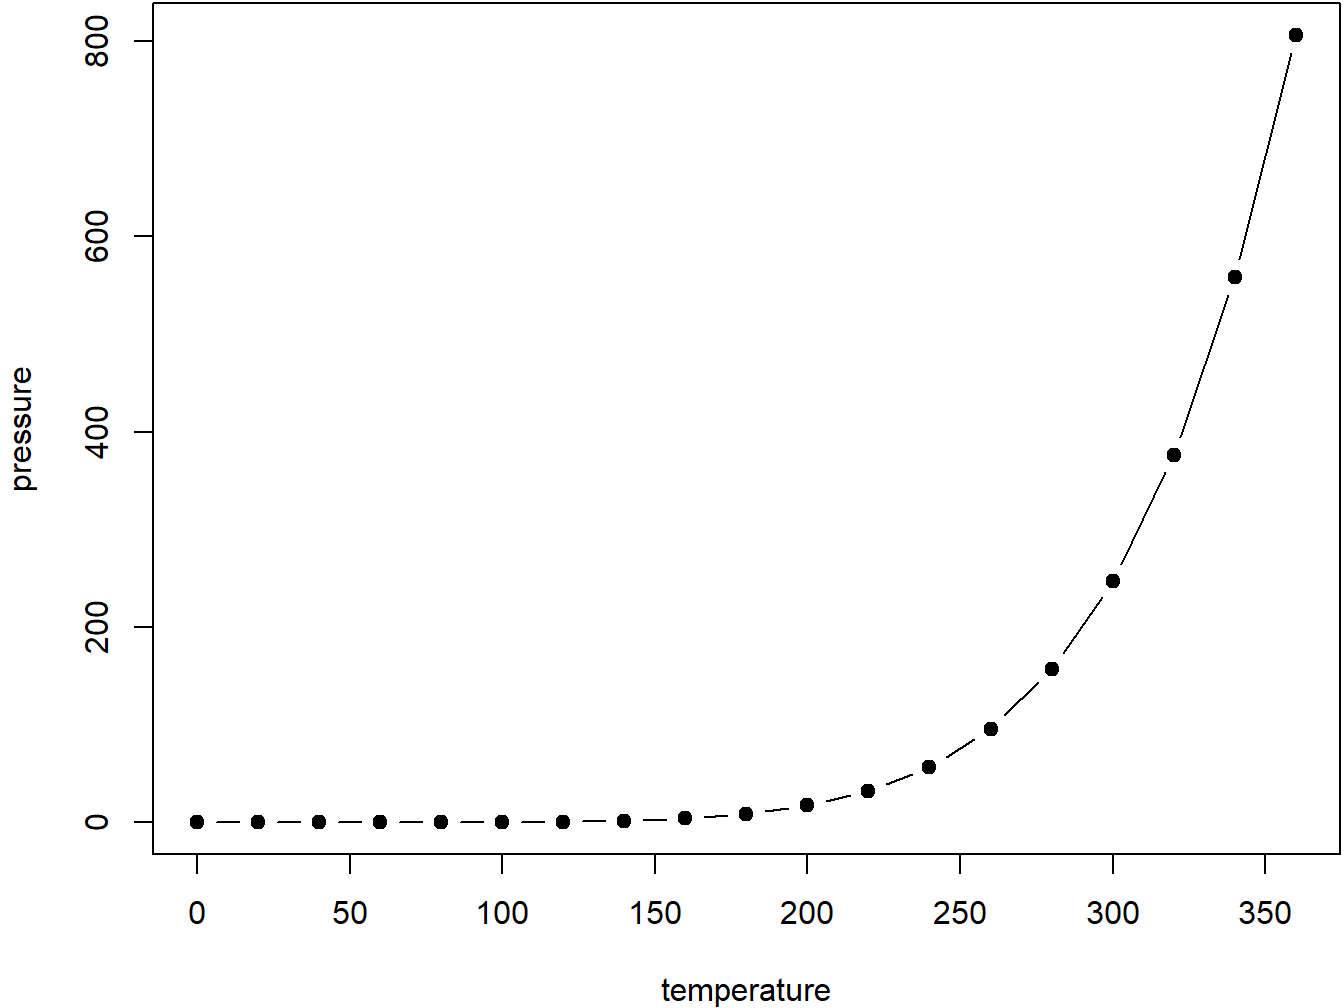
\includegraphics[width=0.8\linewidth]{_main_files/figure-latex/nice-fig-1} 

}

\caption{Here is a nice figure!}\label{fig:nice-fig}
\end{figure}

Don't miss Table \ref{tab:nice-tab}.

\begin{Shaded}
\begin{Highlighting}[]
\NormalTok{knitr}\SpecialCharTok{::}\FunctionTok{kable}\NormalTok{(}
  \FunctionTok{head}\NormalTok{(pressure, }\DecValTok{10}\NormalTok{), }\AttributeTok{caption =} \StringTok{\textquotesingle{}Here is a nice table!\textquotesingle{}}\NormalTok{,}
  \AttributeTok{booktabs =} \ConstantTok{TRUE}
\NormalTok{)}
\end{Highlighting}
\end{Shaded}

\begin{table}

\caption{\label{tab:nice-tab}Here is a nice table!}
\centering
\begin{tabular}[t]{rr}
\toprule
temperature & pressure\\
\midrule
0 & 0.0002\\
20 & 0.0012\\
40 & 0.0060\\
60 & 0.0300\\
80 & 0.0900\\
\addlinespace
100 & 0.2700\\
120 & 0.7500\\
140 & 1.8500\\
160 & 4.2000\\
180 & 8.8000\\
\bottomrule
\end{tabular}
\end{table}

\hypertarget{parts}{%
\chapter{Parts}\label{parts}}

You can add parts to organize one or more book chapters together. Parts can be inserted at the top of an .Rmd file, before the first-level chapter heading in that same file.

Add a numbered part: \texttt{\#\ (PART)\ Act\ one\ \{-\}} (followed by \texttt{\#\ A\ chapter})

Add an unnumbered part: \texttt{\#\ (PART\textbackslash{}*)\ Act\ one\ \{-\}} (followed by \texttt{\#\ A\ chapter})

Add an appendix as a special kind of un-numbered part: \texttt{\#\ (APPENDIX)\ Other\ stuff\ \{-\}} (followed by \texttt{\#\ A\ chapter}). Chapters in an appendix are prepended with letters instead of numbers.

\hypertarget{footnotes-and-citations}{%
\chapter{Footnotes and citations}\label{footnotes-and-citations}}

\hypertarget{footnotes}{%
\section{Footnotes}\label{footnotes}}

Footnotes are put inside the square brackets after a caret \texttt{\^{}{[}{]}}. Like this one \footnote{This is a footnote.}.

\hypertarget{citations}{%
\section{Citations}\label{citations}}

Reference items in your bibliography file(s) using \texttt{@key}.

For example, we are using the \textbf{bookdown} package \citep{R-bookdown} (check out the last code chunk in index.Rmd to see how this citation key was added) in this sample book, which was built on top of R Markdown and \textbf{knitr} \citep{xie2015} (this citation was added manually in an external file book.bib).
Note that the \texttt{.bib} files need to be listed in the index.Rmd with the YAML \texttt{bibliography} key.

The RStudio Visual Markdown Editor can also make it easier to insert citations: \url{https://rstudio.github.io/visual-markdown-editing/\#/citations}

\hypertarget{blocks}{%
\chapter{Blocks}\label{blocks}}

\hypertarget{equations}{%
\section{Equations}\label{equations}}

Here is an equation.

\begin{equation} 
  f\left(k\right) = \binom{n}{k} p^k\left(1-p\right)^{n-k}
  \label{eq:binom}
\end{equation}

You may refer to using \texttt{\textbackslash{}@ref(eq:binom)}, like see Equation \eqref{eq:binom}.

\hypertarget{theorems-and-proofs}{%
\section{Theorems and proofs}\label{theorems-and-proofs}}

Labeled theorems can be referenced in text using \texttt{\textbackslash{}@ref(thm:tri)}, for example, check out this smart theorem \ref{thm:tri}.

\begin{theorem}
\protect\hypertarget{thm:tri}{}\label{thm:tri}For a right triangle, if \(c\) denotes the \emph{length} of the hypotenuse
and \(a\) and \(b\) denote the lengths of the \textbf{other} two sides, we have
\[a^2 + b^2 = c^2\]
\end{theorem}

Read more here \url{https://bookdown.org/yihui/bookdown/markdown-extensions-by-bookdown.html}.

\hypertarget{callout-blocks}{%
\section{Callout blocks}\label{callout-blocks}}

The R Markdown Cookbook provides more help on how to use custom blocks to design your own callouts: \url{https://bookdown.org/yihui/rmarkdown-cookbook/custom-blocks.html}

\hypertarget{sharing-your-book}{%
\chapter{Sharing your book}\label{sharing-your-book}}

\hypertarget{publishing}{%
\section{Publishing}\label{publishing}}

HTML books can be published online, see: \url{https://bookdown.org/yihui/bookdown/publishing.html}

\hypertarget{pages}{%
\section{404 pages}\label{pages}}

By default, users will be directed to a 404 page if they try to access a webpage that cannot be found. If you'd like to customize your 404 page instead of using the default, you may add either a \texttt{\_404.Rmd} or \texttt{\_404.md} file to your project root and use code and/or Markdown syntax.

\hypertarget{metadata-for-sharing}{%
\section{Metadata for sharing}\label{metadata-for-sharing}}

Bookdown HTML books will provide HTML metadata for social sharing on platforms like Twitter, Facebook, and LinkedIn, using information you provide in the \texttt{index.Rmd} YAML. To setup, set the \texttt{url} for your book and the path to your \texttt{cover-image} file. Your book's \texttt{title} and \texttt{description} are also used.

This \texttt{gitbook} uses the same social sharing data across all chapters in your book- all links shared will look the same.

Specify your book's source repository on GitHub using the \texttt{edit} key under the configuration options in the \texttt{\_output.yml} file, which allows users to suggest an edit by linking to a chapter's source file.

Read more about the features of this output format here:

\url{https://pkgs.rstudio.com/bookdown/reference/gitbook.html}

Or use:

\begin{Shaded}
\begin{Highlighting}[]
\NormalTok{?bookdown}\SpecialCharTok{::}\NormalTok{gitbook}
\end{Highlighting}
\end{Shaded}

\hypertarget{sharing-your-book-1}{%
\chapter{Sharing your book}\label{sharing-your-book-1}}

\hypertarget{publishing-1}{%
\section{Publishing}\label{publishing-1}}

HTML books can be published online, see: \url{https://bookdown.org/yihui/bookdown/publishing.html}

\hypertarget{pages-1}{%
\section{404 pages}\label{pages-1}}

By default, users will be directed to a 404 page if they try to access a webpage that cannot be found. If you'd like to customize your 404 page instead of using the default, you may add either a \texttt{\_404.Rmd} or \texttt{\_404.md} file to your project root and use code and/or Markdown syntax.

\hypertarget{metadata-for-sharing-1}{%
\section{Metadata for sharing}\label{metadata-for-sharing-1}}

Bookdown HTML books will provide HTML metadata for social sharing on platforms like Twitter, Facebook, and LinkedIn, using information you provide in the \texttt{index.Rmd} YAML. To setup, set the \texttt{url} for your book and the path to your \texttt{cover-image} file. Your book's \texttt{title} and \texttt{description} are also used.

This \texttt{gitbook} uses the same social sharing data across all chapters in your book- all links shared will look the same.

Specify your book's source repository on GitHub using the \texttt{edit} key under the configuration options in the \texttt{\_output.yml} file, which allows users to suggest an edit by linking to a chapter's source file.

Read more about the features of this output format here:

\url{https://pkgs.rstudio.com/bookdown/reference/gitbook.html}

Or use:

\begin{Shaded}
\begin{Highlighting}[]
\NormalTok{?bookdown}\SpecialCharTok{::}\NormalTok{gitbook}
\end{Highlighting}
\end{Shaded}


  \bibliography{book.bib,packages.bib}

\end{document}
